\documentclass{article}
%\usepackage[a4paper]{geometry}
\usepackage{fullpage}
\usepackage[utf8]{inputenc}
\usepackage[spanish, mexico]{babel}
\usepackage{lipsum}
\usepackage{bm}
\usepackage{upgreek}
\usepackage{enumitem}
\usepackage{mathrsfs}
\usepackage{amsmath}
\usepackage{amssymb}
\usepackage{tikz}
\usepackage{tcolorbox}
\usepackage{csquotes}
\usetikzlibrary{arrows, automata}

\tikzset{
    automaton/.style={
        ->, %arrow type
        >=stealth', %arrow head type (bold)
        shorten >=1pt, 
        auto,
        %semithick,
        initial text=$ $, %no start text
    }
}


% mathtools for: Aboxed (put box on last equation in align envirenment)
\usepackage{microtype} %improves the spacing between words and letters

%% COLOR DEFINITIONS

\usepackage{xcolor} % Enabling mixing colors and color's call by 'svgnames'

\definecolor{MyColor1}{rgb}{0.2,0.4,0.6} %mix personal color
\newcommand{\textb}{\color{Black} \usefont{OT1}{lmss}{m}{n}}
\newcommand{\blue}{\color{MyColor1} \usefont{OT1}{lmss}{m}{n}}
\newcommand{\blueb}{\color{MyColor1} \usefont{OT1}{lmss}{b}{n}}
\newcommand{\red}{\color{LightCoral} \usefont{OT1}{lmss}{m}{n}}
\newcommand{\green}{\color{Turquoise} \usefont{OT1}{lmss}{m}{n}}

\DeclareMathOperator{\trace}{trace}
\DeclareMathOperator{\diag}{diag}

%% FONTS AND COLORS

%    SECTIONS

\usepackage{titlesec}
\usepackage{sectsty}
%%%%%%%%%%%%%%%%%%%%%%%%
%set section/subsections HEADINGS font and color
%\sectionfont{\color{Black}}  % sets colour of sections
%\subsectionfont{\color{Black}}  % sets colour of sections

%set section enumerator to arabic number (see footnotes markings alternatives)
\renewcommand\thesection{\arabic{section}} %define sections numbering
\renewcommand\thesubsection{\thesection\arabic{subsection}} %subsec.num.

%define new section style
\newcommand{\mysection}{
\titleformat{\section} [runin] {\usefont{OT1}{lmss}{b}{n}\color{MyColor1}} 
{\thesection} {3pt} {} } 


% %	CAPTIONS
% \usepackage{caption}
% \usepackage{subcaption}
% %%%%%%%%%%%%%%%%%%%%%%%%
% \captionsetup[figure]{labelfont={color=Turquoise}}


%		!!!EQUATION (ARRAY) --> USING ALIGN INSTEAD
%using amsmath package to redefine eq. numeration (1.1, 1.2, ...) 
\renewcommand{\theequation}{\thesection\arabic{equation}}

\setlength\parindent{0pt}




\makeatletter
\let\reftagform@=\tagform@
\def\tagform@#1{\maketag@@@{(\ignorespaces\textcolor{red}{#1}\unskip\@@italiccorr)}}
\renewcommand{\eqref}[1]{\textup{\reftagform@{\ref{#1}}}}
\makeatother
\usepackage{hyperref}
\hypersetup{colorlinks=true}

% For labeling top of page on every page but first one:
%\usepackage{fancyhdr}

\newcommand{\myclass}{TC1003B -- Modelación de la Ingeniería con Matemática Computacional} % Class name?
\newcommand{\mytitle}{Examen de Módulo} % Title of document?
\newcommand{\mydate}{10.03.2020} % The date?
\newcommand{\myheader}{
    \begin{flushleft}
        \large
        Nombre: \rule{10 cm}{0.4mm} \hfill Matrícula: \rule{2 cm}{0.4mm}\\[1.5ex]
        Nombre: \rule{10 cm}{0.4mm} \hfill Matrícula: \rule{2 cm}{0.4mm}\\[1.5ex]
        Nombre: \rule{10 cm}{0.4mm} \hfill Matrícula: \rule{2 cm}{0.4mm}\\[1.5ex]
        Nombre: \rule{10 cm}{0.4mm} \hfill Matrícula: \rule{2 cm}{0.4mm}
    \end{flushleft}
}

\title{
    \myclass \\
    \textbf{\mytitle} \\
    \myheader
    \date{}
}

% You can set the date automatically by replacing "date goes here" with "\today"

% \renewcommand{\rmdefault}{phv} % Arial Font
% \renewcommand{\sfdefault}{phv} % Arial Font

% \pagestyle{fancy}
% \fancyhead{}
% \fancyhead[CO,CE]{{\small{{\bf{\mytitle}} -- \myclass}}}

\begin{document}
\maketitle

\vspace{-1.5cm}

Lee cuidadosamente y contesta lo que se te pide.
Este examen está pensado para resolverse \textbf{en equipo}, y en poco menos de 90 minutos.
Se sugiere que administres bien tu tiempo.

Al momento de contestar, intenten ser lo más explícito posible: se calificará con base en lo que esté escrito, y se considerará el proceso aún cuando la respuesta final esté errada.
Recuerda que puedes revisar material de la clase, el libro de texto o tus notas.
Buena suerte.

\section{Redes Neuronales (70\%)}

Una red neuronal es un mecanismo de aprendizaje automático muy utilizado en inteligencia artificial que sirve para aproximar funciones usando reconocimiento de patrones.
La función que la red neuronal aproxima puede servir para separar en grupos definidos (clasificación) o bien para predecir comportamientos (regresión).

Para entender cómo funciona una red neuronal, primero es necesario entender cómo funciona cada neurona.

\begin{figure}[htbp]
    \centering
    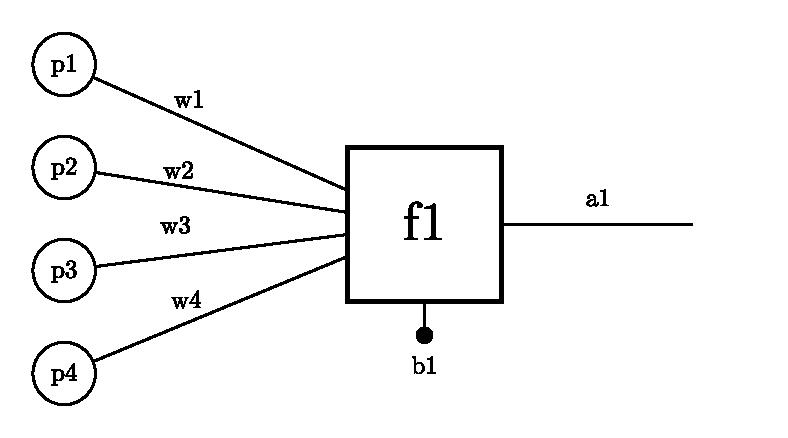
\includegraphics[width=0.6\textwidth]{perceptron.pdf}
    \caption{Perceptrón: una red neuronal de una sola neurona}
    \label{fig:perceptron}
\end{figure}

Un \textbf{perceptrón} es una red neuronal que consta de una sola neurona, como se muestra en la Fig.~\ref{fig:perceptron}.
La neurona recibe señales por una serie de entradas, cuyas conexiones tienen cierto peso o importancia y que, si en conjunto son lo suficientemente \textit{estimulantes}---a pesar de su predisposición sensorial---, se activa y \textit{genera} una reacción.
Podemos representar cada uno de sus componentes con símbolos matemáticos:
\begin{itemize}
    \item Un conjunto de \textbf{entradas} sensoriales $p_j$, donde cada una representa una característica o variable a tomar en cuenta
    \item Un conjunto de \textbf{pesos} $w_{j}$, donde cada uno determina la importancia que cada entrada ejerce sobre la neurona
    \item Una predisposición sensorial o \textbf{sesgo} $b_i$, que es una cantidad que afecta a la capacidad de la neurona para reaccionar a los estímulos
    \item Una \textbf{función de activación} $f_i$, que genera una reacción a los estímulos que percibe
    \item Una \textbf{salida} o reacción $a_i$, que es generada por la neurona dados los estímulos de sus entradas
\end{itemize}



Describe cada uno de los siguientes lenguajes utilizando expresiones regulares genéricas. En dado caso de que el lenguaje no se pueda describir con una ER, menciona por qué. Posteriormente e independientemente de si tienes ER o no, escribe dos ejemplos de palabras aceptadas para cada lenguaje.

\begin{enumerate}[label=\tt \alph*)]
    \itemsep0em
    \item El lenguaje de las palabras en $\{a,b\}$ que empiezan con $a$ y terminan con $b$.
    \item El lenguaje de las palabras en $\{0,1\}$ que son múltiplos de $100$.
    \item El lenguaje de las palabras en $\{x, y\}$ que son de longitud impar o que terminan en $xxx$.
    \item El lenguaje de las palabras en $\{0,1,2\}$ que tengan un $1$ en el centro, y sean simétricas.
    \item El lenguaje de las palabras en $\{z : z \in \mathbb{N}, 0 \leq z \leq 9\}$ que son también denominaciones de billetes o monedas expedidas por el Banco de México y que están en circulación. Omite centavos y series especiales (Onzas de plata, Centenarios, etc.).
    \item El lenguaje de las palabras en $\{a,b\}$ que tengan un número par de $b$s. (\textit{Hint: considera hacer un autómata si te parece muy complicado})
\end{enumerate}


\section{Gramáticas Regulares (14 \% + 6 \%)}

En \texttt{HTML}, le llamamos ``etiquetas'' a las \textit{keywords} para abrir o cerrar elementos de la página web.
Una etiqueta siempre se escribe entre \textit{brackets} para iniciar el elemento, y la misma etiqueta pero con una diagonal al principio para finalizar el elemento.
La etiqueta \verb|<html>...</html>| sirve para delimitar el contenido de la página web.

\begin{enumerate}[label=\tt \alph*)]
    \itemsep0em
    \item Escribe una expresión regular para seleccionar las \textit{keywords} de inicio y fin de las listas ordenadas (\texttt{ol}) y no ordenadas (\texttt{ul}), incluyendo los brackets como parte de la selección (4 \%)
    \item Convierte a AF (5 \%)
    \item Convierte a Gramática \textbf{Regular} (no GLC) (5 \%)
    \item Escribe el árbol de derivación para dos palabras válidas (+ 6\%)
\end{enumerate}


\section{Ambigüedad en GLCs (20\%)}

Sea $G=(\{S\},\{\mathtt{if}, c, \mathtt{then}, \mathtt{else}, x\}, \{S \to x, S \to \mathtt{if} \, c \, \mathtt{then} \, S, S \to \mathtt{if} \, c \, \mathtt{then} \, S \, \mathtt{else} \, S\}, S)$ una gramática libre de contexto.

\begin{enumerate}[label=\tt \alph*)]
    \item Demuestra que $G$ es ambigua utilizando dos árboles de derivación diferentes para una misma frase (10 \%)
    \item Expresa cada árbol de derivación en forma secuencial (usando $\implies$) (10 \%)
\end{enumerate}


\section{Gramáticas Libres de Contexto (30 \% +14 \%)}

El \textit{Biologic Space Lab} está en problemas nuevamente.
Debido a una brecha en un ducto de ventilación, ciertos parásitos lograron entrar a uno de los laboratorios de acceso restringido, en el cual se almacenaban muestras de ADN de especies inteligentes para fines taxonómicos.
Algunos de los bancos de datos están corruptos debido a la infección, pero otros aún están a salvo.
HQ te ha asignado la tarea de diseñar un sistema de control para identificar aquellas muestras de ADN que aún pueden rescatarse, y te ha enviado la siguiente información:

\begin{itemize}
    \itemsep0em
    \item Los parásitos tienen la capacidad de alterar la cadena de ADN, copiando y replicando ciertas subcadenas que consideran necesarias para la supervivencia mediante mutación.
    \item Al parecer, el parásito replica el número de extremidades inferiores y de globos oculares de manera arbitraria.
    \item Utilizando cerca de 20 Petabytes de información, se ha confirmado que el número de réplicas de subcadenas de ADN pertenecientes a los ojos nunca es el mismo que el de las extremidades inferiores en un mismo individuo---en un individuo mutado, el número final de ojos nunca es igual al número final de piernas.
    \item Gracias al análisis de los datos, se determinó también que los parásitos sólo están afectando especies `aptas y balanceadas'; aquellas que tienen el mismo número de ojos que de piernas antes de la mutación.
\end{itemize}

Además, dado a la gran bio-diversidad del BSL, HQ te sugiere lo siguiente:

\begin{tcolorbox}
{\small Tenemos cerca de 900,000 especies en el databank.
Es mejor enfocarse en encontrar las discrepancias en el número de genes en lugar de buscar una secuencia.
Por favor, date prisa. No queremos perder 350 años de trabajo.}
\end{tcolorbox}

Diseña un conjunto de reglas para generar subcadenas de ADN válidas que pudieran estar infectadas. Sugerencias:

\begin{enumerate}[label=\tt \alph*)]
    \item Genera el alfabeto de terminales (2 \%)
    \item Describe (con notación de conjuntos o con palabras) el lenguaje aceptado por tu gramática (5 \%)
    \item Genera las reglas de tu GLC (10 \%)
    \item Describe formalmente tu GLC (5 \%)
    \item Usando tu gramática y sus símbolos y reglas, escribe el árbol de derivación de un \textit{Dachora}, una especie de ave que tiene dos piernas y dos ojos (8 \%)
    \item Dibuja un \textit{Dachora} (+4 \%)
    \item Haz un Autómata de Pila para tu GLC (+10 \%)
\end{enumerate}

\vfill

\textbf{De acuerdo con el Código de Ética del Tecnológico de Monterrey, mi desempeño en esta actividad estará guiado por la integridad académica.}
\end{document}